\documentclass{article}
\usepackage[letterpaper, margin = 1in]{geometry}
\usepackage[usenames, dvipsnames]{color}
\usepackage{graphicx}
\usepackage{amsmath, amssymb}
\usepackage{amsfonts}
\usepackage{cancel}
\usepackage{soul}

\begin{document}

\title{CS229 : Project Milestone}
\author{Jee Ian Tam (jeetam), Sean Rafferty (seanraff)}

\section{Introduction}
There are a large number of open live webcams that are accessible over the
internet. Such webcams can show interesting content from various places all
around the world, but it is not feasible for a single person to browse all of
the webcams to search for such interesting content. Our project aims to use
Machine Learning algorithms to cluster and identify webcams of interest out of
a large pool of webcams.

We scrape a list of publicly accessible, non-password-protected webcams from
opentopia.com. The website provides metadata about the webcam (GPS coordinates,
location name, local time) as well as a URL which can be used to retreive a
snapshot of the most recent image for a webcam. We log images from 2000 webcams
with a 5-minute recording period over a duration of 1 week. The goal is to
train our Machine Learning algorithms on this training data set, and then test
them on the live webcams.

A large majority of webcams at any one time do not display anything
interesting, and simply show a static background. An interest metric that we
can define is a measure of the activity that is occurring as recorded by the
webcam. In order to highlight webcams that have a high interest metric, we use
a background subtraction algorithm combined with some post-processing to detect
foregound objects against the background recorded by the webcam. This is
detailed in section 2.

Another method that we use to explore the data set is to perform K-means
clustering on the webcam images to see if the webcams in the data set can be
meaningfully clustered. For example, in the data set there could be a cluster
of webcams that are located outdoors, a cluster of webcams that show natural
scenery, a cluster of webcams that show images of towns around the world, etc.
\textcolor{red}{[! Sean to add more stuff here about context/results behind
K-means!]}

\section{Clustering}
First, we will discuss what class of categories we are trying to achieve with
our clustering. Then, we describe our method of generating features which are
capable of achieving these categories. Next, we will discuss the choices we
made with respect to modeling the problem and our use of clustering. Finally,
we will present our results and ideas for future improvement.

Our goal is to cluster webcams in ways that people will find both interesting
and useful. Therefore, it wasn't good enough to achieve clusters that are
merely visually obvious (such as simple color-based clustering). Instead, we
wanted to capture semantic information about each webcam and cluster based on
that. To accomplish this, we decided to base our features on image descriptors.
As a brief introduction, an image descriptor is a distinctive vector computed
over a small region of an image. There are many algorithms that detect regions
and extract descriptors in a ``smart'' way. Good detectors find a large number
of descriptors and have a high likelihood of finding the same descriptors in a
scene taken under moderately different conditions (lighting, rotation, scale).
Similarly, good extractors will compute discriptors that are fairly robust to
scale, lighting, and rotation. Together, this means that descriptors extracted
in this way tend to be reliable indicators of complex image features, and
therefore also relaible indicators of basic objects within images.

We are now tasked with converting these descriptors to features. Since each
frame produces a large and varying number of descriptors, and each descriptor
lives in a high-dimensional real space (for example, SIFT descriptors live in
$\mathbb{R}^{128}$), we must find a way to compress these descriptors into a
single vector. To do so, we will use a Bag-of-Features (BoF) model (akin to the
Bag-of-Words model used in text). In this model, we first generate a
$\textit{visual vocabulary}$ by clustering descriptors sampled from each webcam
into a much smaller number of descriptors. Then, we can compute a feature
vector for each webcam by first sampling descriptors from each webcam and then
computing a histogram of the closest descriptors in the visual vocabulary. In
this way, we are left with feature vectors that have the same dimension as the
descriptors we have computed. Once we have these features, we can cluster the
webcams into categories that roughly correspond to the presence of objects.

There are quite a few design decisions within this framework. First, we had to
decide how to sample descriptors from the webcams to both generate the
vocabulary and compute the feature vectors. Additionally, we had to choose
which keypoint detector and descriptor extractor to use. Furthermore, we had to
decide how large we wanted our vocabulary to be and how many webcam clusters we
wanted.  Aside from these modeling choices, we also had to make choices about
the clustering algorithm itself.

To retrieve a set of descriptors from each webcam, we decided to randomly
sample a fixed number of frames (uniformly) from each webcam and extract
descriptors from them. We did this both for generating the visual vocabulary
and for computing the feature vectors. Note that this means that larger or
more-feature rich images are expected to contribute more to the vocabulary and
are also expected to have feautre vectors with larger norms. Although
complexity is something we may be interested in clustering, image size is not.
We address this later in our discussion for improvements.

We experimented with three of the most popular keypoint detectors and
descriptor extractors: SIFT\footnote{D. Lowe, Distinctive Image Features from
  Scale-Invariant Keypoints, Canada, January 2004,
  https://www.cs.ubc.ca/~lowe/papers/ijcv04.pdf}, SURF\footnote{H. Bay, T.
  Tuytelaars, L. Van Gool, SURF: Speeded Up Robust Features,  Zurich, 2006,
  http://www.vision.ee.ethz.ch/~surf/eccv06.pdf}, and FREAK\footnote{A. Alahi,
  R. Ortiz, P. Vandergheynst, FREAK: Fast Retina Keypoint, Switzerland, 2012,
http://infoscience.epfl.ch/record/175537/files/2069.pdf}. According to a
lecture draft\footnote{K. Grauman, B. Leibe, Visual Recognition, 2009,
http://www.cs.utexas.edu/~grauman/courses/fall2009/papers/bag\_of\_visual\_words.pdf},
interest operators (like SIFT, SURF, and FREAK) will provide reasonabily
distinct descriptors for specific objects. However, dense detectors perform
better for category-level tasks. Recall that we've posited that objects are
what we are interested in detecting. However, we are detecting them for the
purpose of categorization. Therefore, we tested the above descriptor extractors
using both their corresponding keypoint detectors as well as a general dense
feature detector (as implemented by OpenCV).

The choice of cluster sizes was fairly experimental. A larger vocabulary gives
you more power, but also increase the risk of overfitting. Similarly, a smaller
vocabulary gives you generalization but may be too weak. We eventually decided
on a vocabulary of size $300$. The number of webcam categories experiences
similar behavior. We wish for the categories to be meaningful (implying more
categories) but also easily distinguishable (implying fewer categories).


For the clustering algorithm itself, we decided to use k-means. This is perhaps
the most popular clustering algorithm and was chosen due to its simplicity,
reasonable runtime, and tendency to produce good results. We experimented with
both random initial clusters and using k-means++ to choose initial clusters,
and found that k-means++ produced significantly better clusters.
\textcolor{red}{TODO(seanrafferty): Experiment with different number of runs of
k-means.}.

\textcolor{red}{TODO(seanrafferty): Results}

\textcolor{red}{TODO(seanrafferty): Suggestions for improvement}


\section{Background Subtraction and Activity Detection}
In order to calculate the interest metric of a webcam, the first step is to
perform background subtraction on the stream of images coming from a webcam.
The goal of this is to effectively detect activity from foreground objects (for
example cars, people, animals, etc.), and to do this it is necessary to train a
classifier to classify foreground objects from the background.

To classifiy foreground objects from the background view of a webcam, we train
each pixel on a Gaussian Mixture Model (GMM) in an unsupervised learning
approach. Each pixel is treated as a vector in the $\mathbb{R}^3$ RGB space,
and is given as input to the GMM to be trained in an online learning method.
The number of Gaussians is adjusted adaptively. We use the
BackgroundSubtractorMOG2() function in the Python OpenCV library to perform
this background subtraction algorithm. The function implements the background
subtraction algorithm as detailed by Z. Zivkovic \footnote{Z.Zivkovic, Improved
adaptive Gausian mixture model for background subtraction, International
Conference Pattern Recognition, UK, August, 2004,
http://www.zoranz.net/Publications/zivkovic2004ICPR.pdf.}.

Initial testing of the interest metric as a function of the number of
classified foreground pixels revealed a flaw in this naive approach : The
foreground detection algorithm suffers from abrupt lighting changes, which
happen very often due to many webcams adjust their aperture dynamically in
response to local lighting conditions. Such occurrences cause the classifier to
erroneously classify a large number of background pixels as foreground. Thus,
this interest metric results in the algorithm giving many false positives,
returning images that had a change in lighting conditions without any
noticeable change in the background or foreground. Thus, this initial approach
did not yield acceptable results. See Figure \ref{Fig:LightingConditions} for
an example.

In order to handle the false positives from this naive implementation, we
introduce an additional post-processing step to reduce the effect of lighting
conditions on the interest metric. Since the foreground detection algorithm
returns a mask where background pixels are colored black and foreground pixels
are colored white, foreground objects show up as white "blobs" against the
black background of the mask. The main observation (or assumption) is that the
blobs of objects of interest (e.g. cars, people, animals, etc.) are small
relative to the size of the image. Thus, if we can base our interest metric on
some function of the blobs and threshold the blobs based on their size, we can
improve the background subtraction pipeline's ability to handle changes in
lighting condition.

We use the SimpleBlobDetector() function in the Python OpenCV library to fit
contours around each blob, and threshold each blob based on a maximum
percentage (nominally 20\%) of the total image area. Furthermore, we now define
the interest metric to be a function of the total area of blobs that occupy an
image foreground. This has the effect of assigning more weight to foreground
objects that are more prominent (have larger area) in the webcam image, which
is what is desired. Adding this post-processing step and redefining the
interest metric to be a function of the total area of blobs results in an
improved webcam highlighting algorithm that is more robust to lighting changes
in webcams. See Figure \ref{Fig:ForegroundDetection} for an example.

Even though we have made the webcam highlighting more robust against lighting
changes, it is still not robust against webcams that move around, causing the
background to shift constantly. The resulting background model from the
background subtraction algorithm is not representative of the actual background
that the webcam is pointing at, resulting in poor object detection performance.
One possible way to address this would be to use the blob detection
post-processing step above to check if a large portion of the image has
changed, and block or refresh the background model to take into account that
the background has changed.

Another improvement that can be made to the interest metric is to take into
include the element of time into the calculation. Currently the webcams are
highlighted based on the current webcam image that has the highest foreground
blob areas, without consideration for the past history of the webcams. However,
one possible way to improve the performance of the webcam highlighting might be
to factor in the frequency and/or duration of the observed activity - That is,
highlight a webcam only when we observe sustained activity over a pre-defined
duration of time. 

\section{Further Work}
In light of the results of our two efforts, we will begin work on labeling
moving objects. Since the results of activity detection are promising, we can
extract moving objects from frames by extracting a small patch containing the
object. Then, we can feed these small patches to an image classifier which will
label the object (e.g. ``vehicle'', ``human'', ``animal'', etc.). Experimenting
with different classifiers will be the most challenging part of this extension.
We will begin with two main approaches. First, we will use the same
Bag-of-Features model that we used in clustering.  Second, we will use a
convolutional neural network. Since we are only interested in moving objects,
our target space is greatly reduced. We do not foresee any need to detect more
than five (and certainly no more than ten) different classes of objects. To
train these models, we will use another labeled dataset containing objects we
are interested in detecting, as well as negative examples. As a sepcialization
to our task, we plan to focus on images that are observed by our motion
detector to have a high false-positive rate (e.g. clouds, water, etc.).

We believe this extension will provide many benefits to our original goal:
finding interesting and similar webcams. First, knowing the density of moving
objects in each webcam enables another method of clustering which has strong
semantic power. Similarly, users can search through webcams to find objects
they are interested in. Additionally, having a classifier that can provide
strong negative classifications (i.e. there are no interesting objects in the
given patch) can help reduce the number of false positives reported by the
motion detector.

\newpage

\section{Appendix}
\begin{figure}[h]
\centering
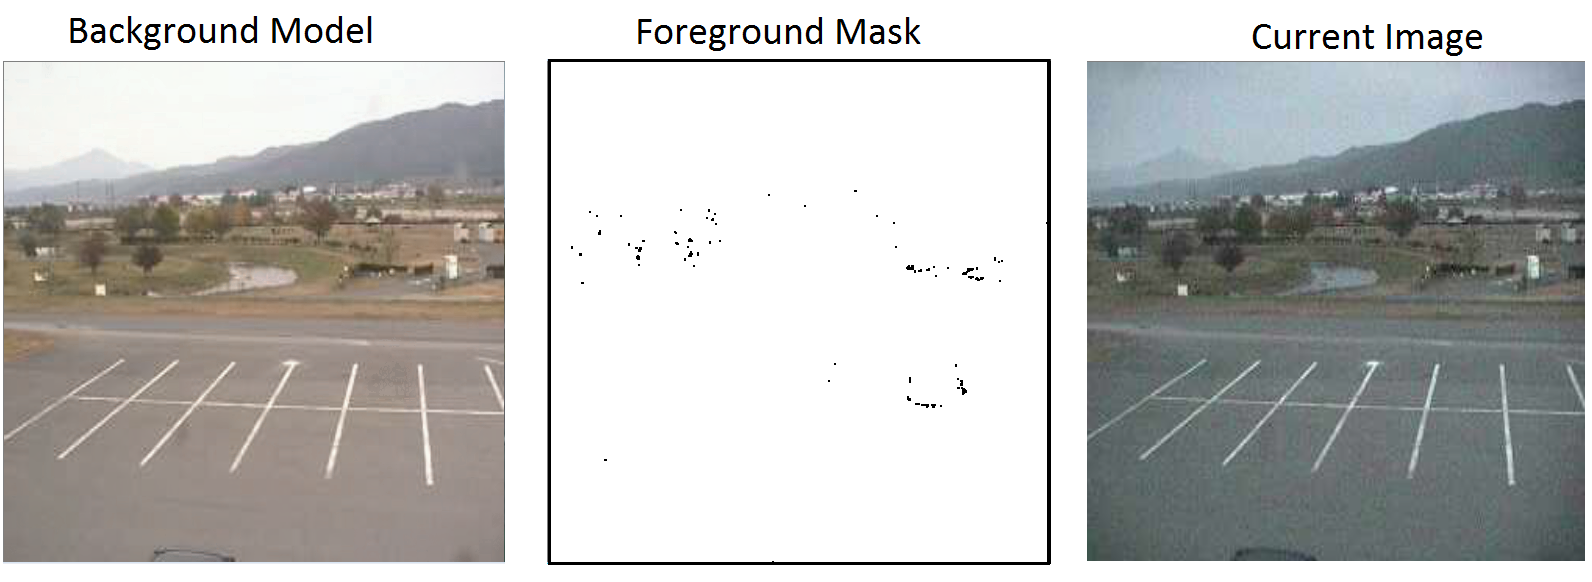
\includegraphics[scale = 0.4]{LightingConditions}
\caption{Failure of Naive background subtraction model to handle lighting changes}
\label{Fig:LightingConditions}
\end{figure}
\begin{figure}[h]
\centering
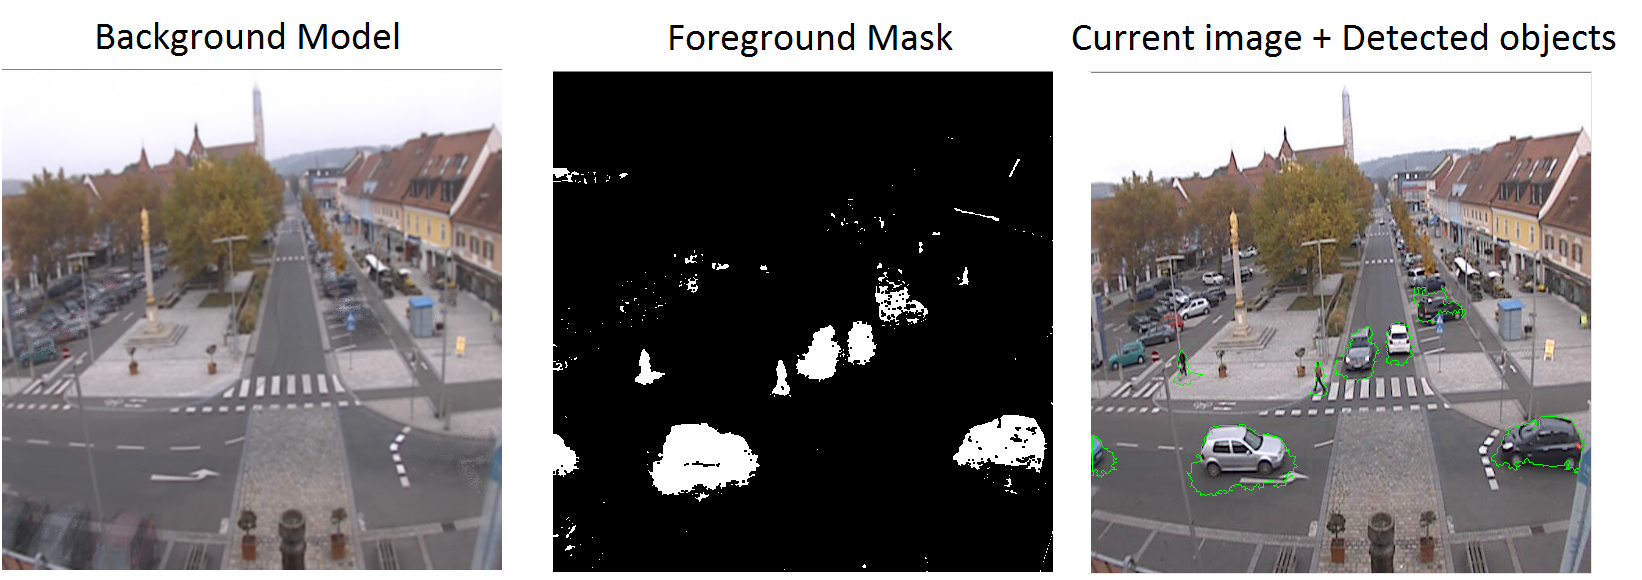
\includegraphics[scale = 0.4]{BackgroundSubtraction1}
\caption{Example of background/foreground segmentation algorithm}
\label{Fig:ForegroundDetection}
\end{figure}






\end{document}
